\section{Evaluation} \label{eval}

\begin{figure*}[h!]
	\centering
	\subfigure[Real time required to encode a tiled configuration for 30~seconds of 3840x2048 video. The encoding process is CPU-bound because tiles a rearranged by the CPU.]{
		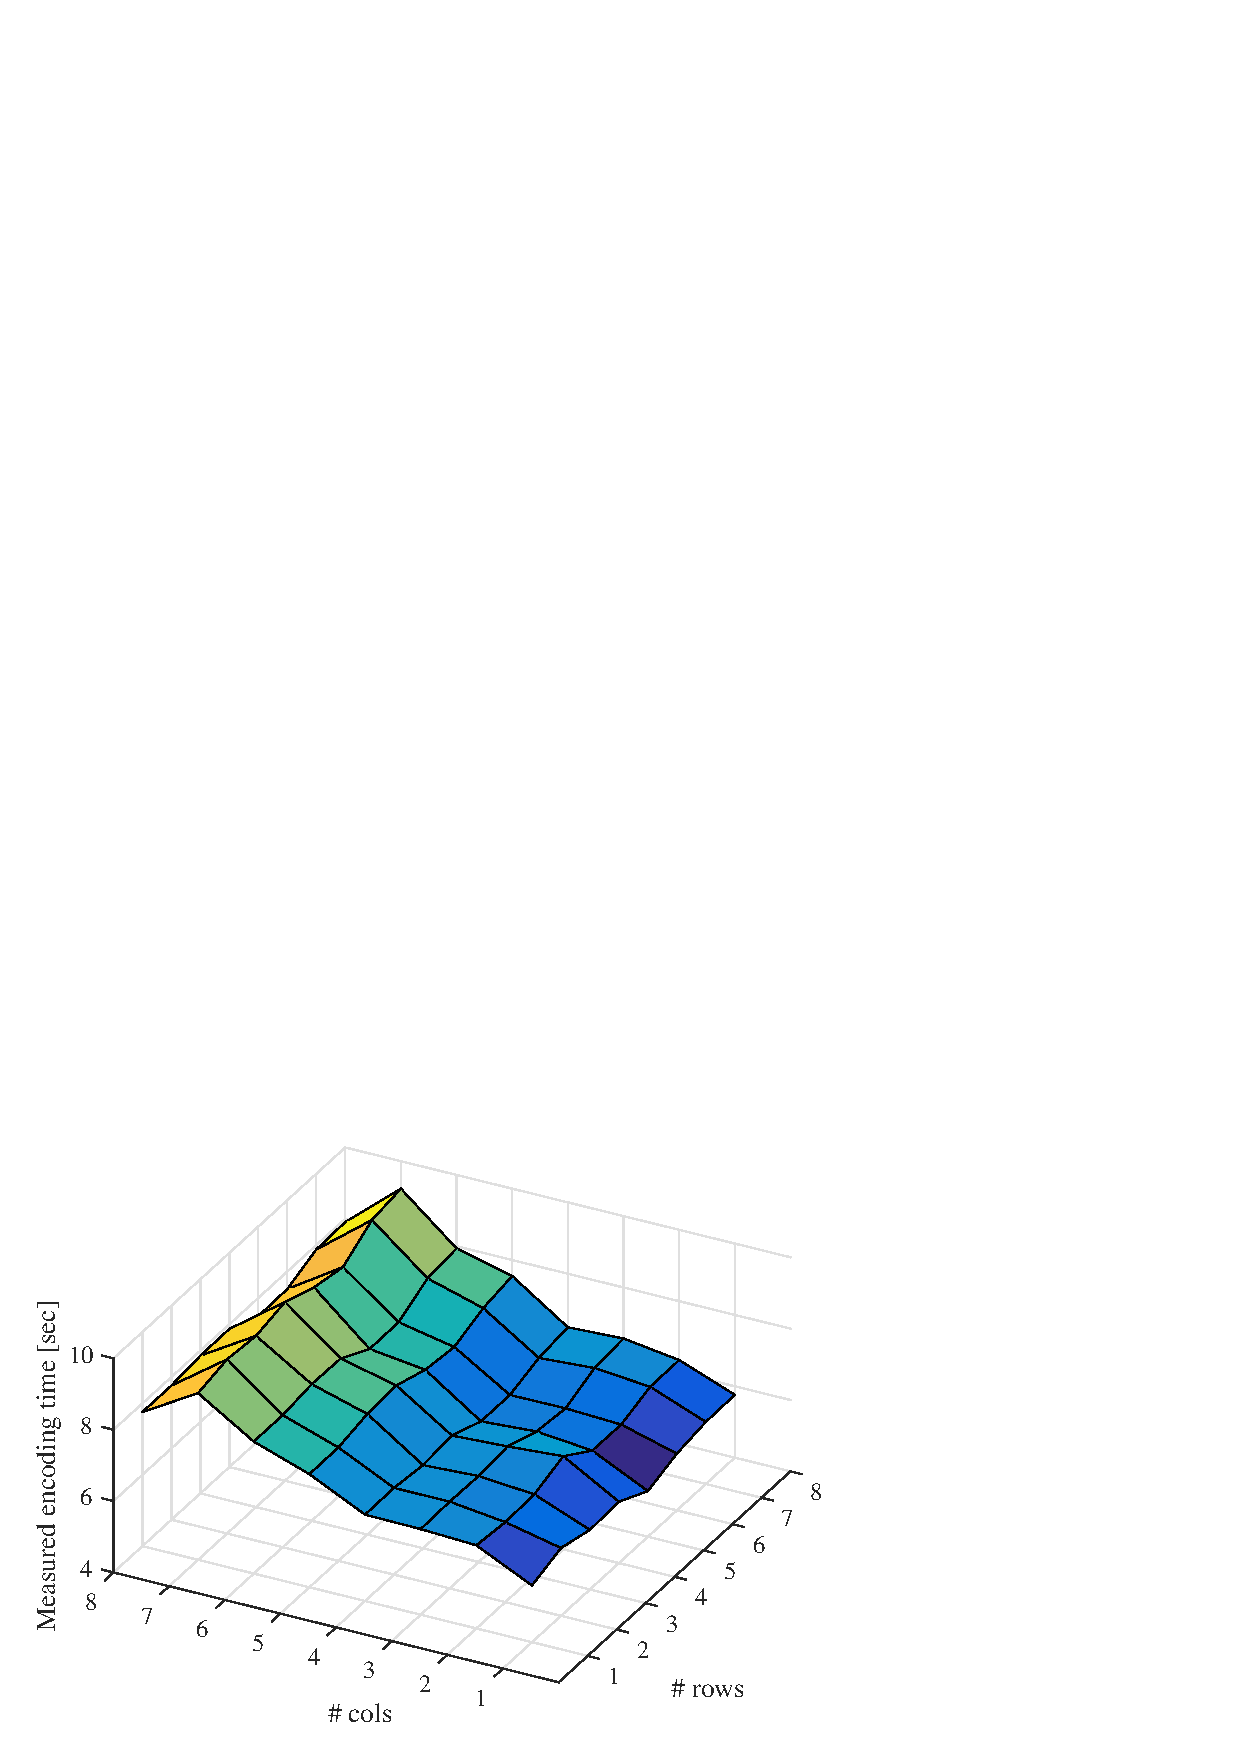
\includegraphics[width=.31\textwidth]{../figures/times_v1.pdf}
		\label{fig:time}
	}
    \hfill
	\subfigure[Sizes of the encoded tiled videos. The video size grows rapidly when additional encoding contexts are required.]{
		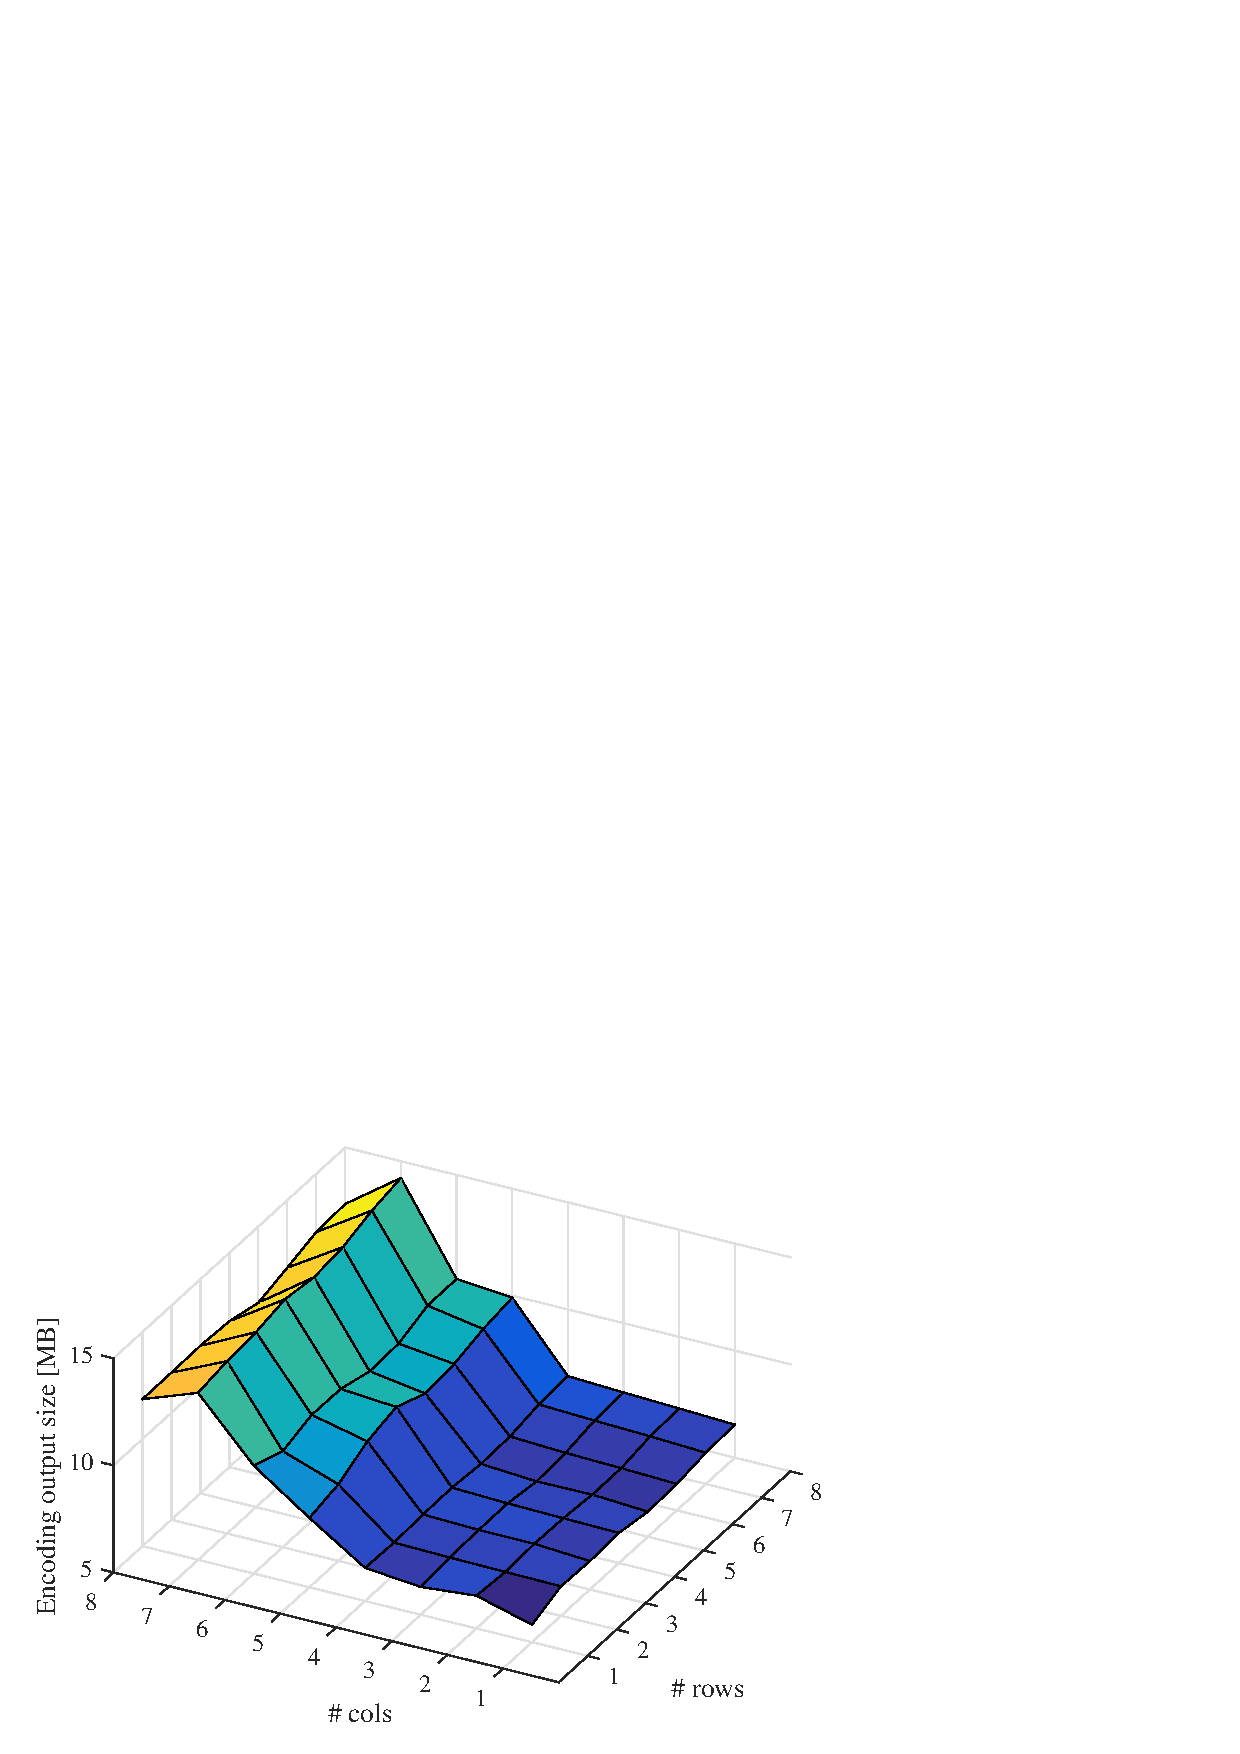
\includegraphics[width=.31\textwidth]{../figures/sizes_v1.pdf}
		\label{fig:size}
	}
    \hfill
	\subfigure[SSIM scores between input and tiles video. "Middle" quality uses a checkerboard pattern. Hardware alignment rules require padding for 3, 5, 6 and 7 rows; 5 and 8 rows are given as representative examples.
 %Other rows are well-aligned; 8 rows are given as example
 ]{
		\includegraphics[width=.31\textwidth]{../figures/ssim_printed.pdf}
		\label{fig:ssim}
	}	
	\caption{Evaluation results on a 30 second video with a resolution of $3840\times2048$ pixels. High and low bitrates are 1.6Mbps and 0.8Mbps, corresponding to 480p and 360p video, respectively.\protect\footnotemark}
	\label{fig:eval}
\end{figure*}
To evaluate RATS, we analyze its performance across multiple tile configurations. In particular, we consider the encoding speed, output file size, and the quality of the final image.
%
Examining Figs.~\ref{fig:time} and \ref{fig:size}, we see that the number of tile columns is the primary factor affecting encoder performance. Note that the number of columns dictates how many sub-images are necessary, each of which requires two more NVENC encodes per frame, multiple stitching operations, and column stacking of the source image. In contrast, the hardware encoder supports tile rows using slice mode 3. Slice mode 3 incurs additional computation costs only when alignment rules force us to crop the source image.

Fig.~\ref{fig:time} confirms that RATS easily satisfies our real-time requirement, finishing the encode and stitch process in one-third of the total video time in the worst case tested.
The small jump from 1 to 2 columns is due to a required source image transformation, both before encoding and afterwards in stitching.
The larger jump from 4 to 5 columns happens when the stacked height reaches the hardware limit, and rearrangements are more severe because another hardware encoder instance is required.
The rapid increase thereafter happens within NVENC, obfuscating its origin.
It is likely a byproduct of the in-loop deblocking filter, which crosses tile boundaries but cannot do this efficiently in the increasingly tall and slim configurations. Configurations of 7 columns incur the worst case padding overhead, making it a particularly challenging case.

% The first notable point in the figure is the jump between 1 and 2 tile columns as the source image requires transformation and the stitcher begins to make more significant bitstream modifications. Another is the jump between 4 and 5 tile columns as sub-images are introduced.
% The gradual increase thenceforth occurs entirely within NVENC, unfortunately obfuscating its origin, but is likely a byproduct of the in-loop deblocking filter becoming less able to process tile boundaries in parallel as the image becomes taller and slimmer. The extra time at 7 columns similarly occurs within NVENC, and is likely due to the CTU width of the uncropped image not being divisible by 7, resulting in inferior alignment.

In Fig.~\ref{fig:size}, we see that the number of columns has a drastic effect on the output file size once sub-images are introduced. Decrease in coding efficiency is to be expected with smaller tiles due to intra-picture prediction and entropy encoding, but it is interesting that this only occurs with sub-images and is not affected by the number of tile rows.
This may also result from the in-loop deblocking filter.
Here too, the spike at 7 columns is likely due to inferior alignment.

In addition to having sufficient speed and coding efficiency, we must ensure that the video quality is good enough to achieve a high quality of experience for the end user.
In a tile-based ABR streaming scenario, this is especially true in high-quality tiles since these will likely be at the current position of the viewport.
Furthermore, NVENC is a new technology not yet capable of matching the output quality of software encoders, and we can expect quality to degrade with more tiles because intra-prediction and motion estimation cannot pass tile boundaries, so choosing an appropriate tile granularity is essential.
We use SSIM to express the deviation between the original and the tiled encoded frames, showing the results in Fig.~\ref{fig:ssim}.
Well-aligned tile configurations (1, 2, 4 and 8 rows, 1 through 6 colums) provide an intuitive quality degradation from high to low quality. In Fig.~\ref{fig:ssim} we only show the representative cases of 5 and 8 rows. For the middle quality we use a checkerboard pattern of alternating low and high qualities per tile showing the maximum number of quality transitions possible. Note that forced alignment of the tile height by cropping requires interpolation before SSIM, with the result that lower quality images with higher blur scores better in SSIM. Configurations with 7 and 8 columns require horizontal padding, resulting in very low SSIM scores.

\footnotetext{https://support.google.com/youtube/answer/2853702}

